%\documentclass{beamer}

\documentclass[10pt]{beamer} 
\usetheme[pageofpages=of,% String used between the current page and the
          % total page count.
          alternativetitlepage=true,% Use the fancy title page.
          %titlepagelogo=coca,% Logo for the first page.
          titleline=true
          ]{Torino}
%\usetheme{Frankfurt}
\usecolortheme{chameleon}

\usepackage{graphicx,hyperref,url}
\usepackage[utf8]{inputenc}
\usepackage[T1]{fontenc}
\usepackage[portuges,brazilian]{babel}
%%%\usepackage{wrapfig}
\usepackage{caption}
\usepackage{subfigure}
%\usepackage{subcaption}
\usepackage{latexsym}
\usepackage{amssymb, amsmath}
\usepackage{multicol}
\usepackage{pifont}%,bbding}%%,dingbat} %%% ver manual de simbolos
\usepackage[final]{listings}
\usepackage{comment}


\definecolor{azulclaro}{rgb}{0.9,0.9,0.9}
\definecolor{mygreen}{rgb}{0,0.6,0}
\definecolor{mygray}{rgb}{0.5,0.5,0.5}
\definecolor{mymauve}{rgb}{0.58,0,0.82}
\definecolor{darkgray}{rgb}{.4,.4,.4}
\definecolor{purple}{rgb}{0.65, 0.12, 0.82}

\newcommand{\minizinc}{MiniZinc}

\lstset{ 
  %  label={pgm_ex01},
    backgroundcolor=\color{azulclaro}, 
    language=erlang, %%Miranda,%%Perl,%%%Python, %%Mercury,
    showstringspaces=false,
    basicstyle=\bf\scriptsize\ttfamily,
%%      basicstyle= \footnotesize %%% TESTAR
%%      keywordstyle=\bfseries\color{green!40!black},
    keywordstyle=\textbf{\color{mygreen}}, 
    otherkeywords={*, \%, array, constraint, solve, output,  show, "/\", satisfy, set, of, if, then, elseif, float, search},
%%  keywordstyle=\color{blue},       % keyword style
%%    commentstyle=\itshape\color{purple!40!black},
      commentstyle=\color{orange},    % comment style
      identifierstyle=\color{blue},
      stringstyle=\color{orange},
      stringstyle=\color{mymauve},
      numbers=left,  % where to put the line-numbers; possible values are (none, left, right)
      numbersep=5pt,   % how far the line-numbers are from the code
      numberstyle=\tiny\color{magenta},
      keepspaces=true      
    % %caption={LEGENDA no source PASCAL ficou OK},
}


\graphicspath{{/home/ccs/Dropbox/figs_genericas/}{figuras/}{/home/ccs/Dropbox/CCS/picat/}}
\DeclareGraphicsExtensions{.pdf,.png,.jpg}
%Global Background must be put in preamble
%\usebackgroundtemplate{\includegraphics[width=\paperwidth]{amarelinho.pdf}}
%%% \begin{frame}[allowframebreaks=0.8]

% The log drawn in the upper right corner.

%\logo{\centering
%\includegraphics[height=0.050\paperheight]{figuras/logo_SBPO_Peixe.png}
%%\hspace{9.6cm}
%\includegraphics[height=0.027\paperheight]{figuras/logo_udesc_horizontal.jpg}


%%%%%%%%%%%%%%%%%%%%%%%%%%%%%%%%%%%%%%%%%%%%%%%%%%%%%%%%%%%%%%%%%%%%%


\title[Picat]{\fontsize{20}{30}\selectfont \textcolor{black}{PICAT: uma Linguagem Multiparadigma}}

\author[Battisti \& PV]{Claudio Cesar de Sá, Rogério Eduardo da Silva, Alexandre Gonçalves, 
    João Herique Faes Battisti, Paulo Victor de Aguiar\\\medskip
    {\small \url{joaobattisti@gmail.com}} \\ 
    {\small \url{pavaguiar@gmail.com}}\\
     {\small \url{claudio.sa@udesc.br}}}

\institute[UDESC]{
    Departamento de Ci\^encia da Computa\c{c}\~ao \\
    Centro de Ci\^encias e Tecnol\'ogias\\
Universidade do Estado de Santa Catarina}

%%%%%%%%%%%%%%%%%%%%%%%%%%%%%%%%%%%%%%%%%%%%%%%%%%%%%%%%%%%%%%%%%%%%%

\begin{document}


\begin{frame}
    \titlepage
\end{frame}

%%%%%%%%%%%%%%%%%%%%%%%%%%%%%%%%%%%%%%%%%%%%%%%%%%%%%%%%%%%%%%%%%%%%%

\begin{frame} [allowframebreaks=0.8]
\frametitle{Sumário}
\tableofcontents
\end{frame}

%%%%%%%%%%%%%%%%%%%%%%%%%%%%%%%%%%%%%%%%%%%%%%%%%%%%%%%%%%%%%%%%%%%%%

\begin{frame}[fragile]
\frametitle{Agradecimentos}
\begin{itemize}
  \item 
  \item Ao Google Images ... vários autores
  
\end{itemize}

\end{frame}



%%%%%%%%%%%%%%%%%%%%%%%%%%%%%%%%%%%%%%%%%%%%%%%%%%%%%%%%%%%%%%%%%%%%%


%%%%%%%%%%%%%%%%%%%%%%%%%%%%%%%%%%%%%%%%%%%%%%%%%%%%%%%%%%%%%%



\section{Introdução}
\begin{frame}

    \frametitle{Histórico}

    \begin{itemize}
      \item Criada em 2013 por Neng-Fa Zhou e Jonathan Fruhman 

      \item Utiliza o B-Prolog como base de implementação, e ambas utilizam 
      a  programação em lógica: Lógica de Primeira-Ordem (LPO)

      \item Uma evolução ao Prolog após seus mais de 40 anos de sucesso!

      \item Sua atual versão é a 2.0 (\today)

    \end{itemize}
\end{frame}

%%%%%%%%%%%%%%%%%%%%%%%%%%%%%%%%%%%%%%%%%%%%%%%%%%%%%%%%%%%%%%%%%%%%%

%\section{Isso é outra seção}
\begin{frame}
    \frametitle{O que é multiparadigma?}

    \begin{itemize}
      \item Imperativo -- Procedural
      \item Funcional
      \item \underline{Lógico}
      \item Uma boa \textit{mistura} de: Haskell, Prolog e Python

    \end{itemize}

\end{frame}

%%%%%%%%%%%%%%%%%%%%%%%%%%%%%%%%%%%%%%%%%%%%%%%%%%%%%%%%%%%%%%%%%%%%%

\begin{frame}
    \frametitle{Algumas Características:}

    \begin{itemize}
    
      \item Sintaxe $\Rightarrow $ elegância do código
      \item Velocidade de execução
      \item Portabilidade (todas plataformas)
      \item Extensão há outras ferramentas
      
    \end{itemize}
\end{frame}

%%%%%%%%%%%%%%%%%%%%%%%%%%%%%%%%%%%%%%%%%%%%%%%%%%%%%%%%%%%%%%%%%%%%%


%%%%%%%%%%%%%%%%%%%%%%%%%%%%%%%%%%%%%%%%%%%%%%%%%%%%%%%%%%%%%%%%%%%%%

\section{Características}
\begin{frame}
    \frametitle{Anacrônico de \textbf{P.I.C.A.T.}}
  
 \begin{description}
   
 
 \item [\textbf{P}:] \textit{Pattern-matching}:  Utiliza o conceito de \textit{casamento padrão}
 equivalente aos conceitos de \textit{unificação} da LPO
 
 \item [\textbf{I}:] \textit{Intuitive}: oferece estruturas de decisão, atribuição e 
 laços de repetição, etc, análogo as outras linguagens de programação
 
  \item [\textbf{C}:] \textit{Constraints}: suporta a Programação por Restrições (PR)
 
     \item [\textbf{A}:] \textit{Actors}: suporte as chamadas a eventos, os atores (futuro gráfico) 
 
  \item [\textbf{T}:] \textit{Tabling}: implementa a técnica de \textit{memoization}, com soluções imediatas para problemas de Programação Dinâmica (PD).
   
  
\end{description}
\end{frame}

%%%%%%%%%%%%%%%%%%%%%%%%%%%%%%%%%%%%%%%%%%%%%%%%%%%%%%%%%%%%%%%%%%%%%

%%%%%%%%%%%%%%%%%%%%%%%%%%%%%%%%%%%%%%%%%%%%%%%%%%%%%%%%%%%%%%%%%%%%%
\subsection{Instalação}
\begin{frame}
    \frametitle{Instalação do PICAT}

  \begin{itemize}
    \item Baixar a versão desejada de \url{http://picat-lang.org/download.html}
   \item Descompactar. Em geral em \textbf{/usr/local/Picat/}
    \item Criar um link simbólico (linux) ou atalhos (Windows):\\ 
   \texttt{ln -s /usr/local/Picat/picat   \hspace{1cm}   /usr/bin/picat}
    \item Se quiser adicionar (opcional) uma variável de ambiente:\\
          \texttt{PICATPATH=/usr/local/Picat/}\\
          \texttt{export PICATPATH}

    \item ou ainda adicione o caminho: \texttt{PATH=\$PATH:/usr/local/Picat}

   \item Finalmente, tenha um editor de código de programa.\\
     Sugestão: \textit{geany} ou \textit{sublime}
     
    \item Escolha a sintaxe da linguagem \textit{Erlang} 
    
  \end{itemize}



\end{frame}

%%%%%%%%%%%%%%%%%%%%%%%%%%%%%%%%%%%%%%%%%%%%%%%%%%%%%%%%%%%%%%%%%%%%%


%%%%%%%%%%%%%%%%%%%%%%%%%%%%%%%%%%%%%%%%%%%%%%%%%%%%%%%%%%%%%%%%%%%%%
\subsection{Usando do Picat}

\begin{frame}
    \frametitle{Usando do Picat}
    \begin{itemize}
     \item Picat é uma linguagem de multiplataforma, disponível em qualquer arquitetura de processamento e também de sistema operacional. Nesta vídeo-aula: Linux (Manjaro)
     \item Em seus arquivos fontes utiliza a extensão \textbf{.pi}. Exemplo: \texttt{programa.pi}
     \item Existem 2 modos de utilização do Picat: modo linha de comando (ou console) e modo interativo
     \item Códigos executáveis 100\% \textbf{stand-alone}: ainda não!
     \item Neste quesito, estamos em igualdade com Java, Prolog e Python
     
    \end{itemize}
\end{frame}

%%%%%%%%%%%%%%%%%%%%%%%%%%%%%%%%%%%%%%%%%%%%%%%%%%%%%%%%%%%%%%%%%%%%%

%%%%%%%%%%%%%%%%%%%%%%%%%%%%%%%%%%%%%%%%%%%%%%%%%%%%%%%%%%%%%%%%%%%%%
\section{Exemplo}
\begin{frame}
    \frametitle{Fatos e Regras -- os pais!}
    \begin{itemize}
    
    \item $pai(platao, luna)$ \hspace{1.5cm} leia-se: \textit{Platão é o pai de Luna}
    \item $pai(platao, péricles)$ \hspace{1.5cm} leia-se: \textit{Platão é o pai de Péricles}
    \item $pai(epimenides, platao)$ \hspace{1.5cm} leia-se: \textit{Sócrates é o pai de Platão}
    \item Codificando tudo isto  em Picat
    \end{itemize}
\end{frame}

\begin{frame}[allowframebreaks=0.9]
 \frametitle{Regras em PICAT}

\lstinputlisting{../regras_ex_02.pi}

\end{frame}


%%%%%%%%%%%%%%%%%%%%%%%%%%%%%%%%%%%%%%%%%%%%%%%%%%%%%%%%%%%%%%%%%%%%%

\section{Tipos de Dados}

\begin{frame}
\frametitle{Tipos de Dados}
\begin{figure}[!ht]
\centering
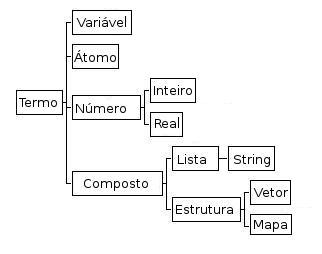
\includegraphics[width=.6\textwidth]{figures/tipos_dados_picat_traduzido.jpg}
\caption{Hierarquia dos Tipos de dados}
\label{Hiera}
\end{figure}
\end{frame}

%%%%%%%%%%%%%%%%%%%%%%%%%%%%%%%%%%%%%%%%%%%%%%%%%%%%%%%%%%%%%%%%%%%%%

%%%%%%%%%%%%%%%%%%%%%%%%%%%%%%%%%%%%%%%%%%%%%%%%%%%%%%%%%%%%%%%%%%%%%
\subsection{Outros Detalhes}
\begin{frame}
    \frametitle{Número}
    \texttt{Picat> A = 5, B = 7, number(A), number(B),
    max(A, B) = Maximo, min(A, B) = Minimo.}\\
  
    \texttt{A = 5}\\
    \texttt{B = 7}\\
    \texttt{Maximo = 7}\\
    \texttt{Minimo = 5}\\
    \texttt{yes.}
\end{frame}

%%%%%%%%%%%%%%%%%%%%%%%%%%%%%%%%%%%%%%%%%%%%%%%%%%%%%%%%%%%%%%%%%%%%%


%%%%%%%%%%%%%%%%%%%%%%%%%%%%%%%%%%%%%%%%%%%%%%%%%%%%%%%%%%%%%%%%%%%%%


%%%%%%%%%%%%%%%%%%%%%%%%%%%%%%%%%%%%%%%%%%%%%%%%%%%%%%%%%%%%%%%%%%%%%

\begin{frame}
    \frametitle{Atribuição}
     \texttt{Picat> X := 7, X := X + 7, X := X + 7.}\\
     \texttt{X = 21}
\end{frame}

%%%%%%%%%%%%%%%%%%%%%%%%%%%%%%%%%%%%%%%%%%%%%%%%%%%%%%%%%%%%%%%%%%%%%

\begin{frame}
    \frametitle{Estruturas de Controle}
        
     \lstinputlisting{../estrutura_if_then_ex01.pi}
    
\end{frame}

%%%%%%%%%%%%%%%%%%%%%%%%%%%%%%%%%%%%%%%%%%%%%%%%%%%%%%%%%%%%%%%%%%%%%

\begin{frame}
    \frametitle{Entradas e Saídas}
  
  
  \lstinputlisting{../media_2_reais.pi}
  
\end{frame}
%%%%%%%%%%%%%%%%%%%%%%%%%%%%%%%%%%%%%%%%%%%%%%%%%%%%%%%%%%%%%%%%%%%%%

%%%%%%%%%%%%%%%%%%%%%%%%%%%%%%%%%%%%%%%%%%%%%%%%%%%%%%%%%%%%%%%%%%%%%

%%%%%%%%%%%%%%%%%%%%%%%%%%%%%%%%%%%%%%%%%%%%%%%%%%%%%%%%%%%%%%%%%%%%%
%%%%%%%%%%%%%%%%%%%%%%%%%%%%%%%%%%%%%%%%%%%%%%%%%%%%%%%%%%%%%%%%%

\section{Conclusão}
\begin{frame}
    \frametitle{Conclusão}
    \begin{itemize}
    \item PICAT é uma linguagem nova (2013), 
    desconhecida, revolucionária e com um futuro promissor
    
    \item Atualmente há pouco material disponível e uma comunidade pequena de usuários

    \item Uso muito bom quanto a: Planejamento, Programação por Restrição e PD (diretamente)
    
    \item Todos problemas NPs-Completos!
    \end{itemize}
\end{frame}

%%%%%%%%%%%%%%%%%%%%%%%%%%%%%%%%%%%%%%%%%%%%%%%%%%%%%%%%%%%%%%%%%%%%%

%\section{Referências}
\begin{frame}
    \frametitle{Referências}
    \begin{itemize}
    \item O \textit{User Guide} que está no diretório  \texttt{doc/} da instalação em \LaTeX
    
     \item Meu GitHub $\Rightarrow $  \url{https://github.com/claudiosa/CCS/tree/master/picat}

     \item \url{http://pic at-lang.org/} -- \textit{User Guide on-line} está lá
    
    \item Assinem o fórum do PICAT(em inglês: respondo lá também)

    \item Site do Hakan  Kjellerstrand  $\Rightarrow $ \url{http://www.hakank.org/picat/}
    \item Site do Roman Barták  $\Rightarrow $ 	\url{http://ktiml.mff.cuni.cz/~bartak/}
    \item Site do Sergii Dimychenko  $\Rightarrow $ \url{http://sdymchenko.com/blog/2015/01/31/ai-planning-picat/}
    
    \end{itemize}
\end{frame}

%%%%%%%%%%%%%%%%%%%%%%%%%%%%%%%%%%%%%%%%%%%%%%%%%%%%%%%%%%%%%%%%%%%%%
 % cap 1


%%%%%%%%%%%%%%%%%%%%%%%%%%%%%%%%%%%%%%%%%%%%%%%%%%%%%%%%%%%%%%
\section{Contexto dos Tipos de Dados}

\begin{frame}
\frametitle{Contexto dos Tipos de Dados}

\begin{itemize}
 

  \item Tipos de dados $\neq  $ estruturas de dados

\item Lembrar que: predicados apresentam valores  V (\texttt{yes}) ou F (\texttt{no}) e funções retornam valores

  \item \textit{Funções} em PICAT são análogas as funções das LPs clássicas

  \item \textit{Predicados} análogo a LPO, a Prolog e seus derivados
 \end{itemize}

\end{frame}

%%%%%%%%%%%%%%%%%%%%%%%%%%%%%%%%%%%%%%%%%%%%%%%%%%%%%%%%%%%%%%
\section{Tipos de Dados}

\begin{frame}
\frametitle{Tipos de Dados}

\begin{figure}[!ht]
\centering
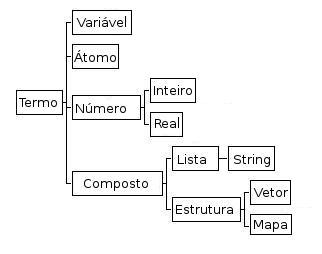
\includegraphics[width=.6\textwidth]{figures/tipos_dados_picat_traduzido.jpg}
\caption{Hierarquia dos tipos de dados $=$ termos}
\label{Hiera}
\end{figure}

\end{frame}

%%%%%%%%%%%%%%%%%%%%%%%%%%%%%%%%%%%%%%%%%%%%%%%%%%%%%%%%%%%%%%%%%%%%%
\subsection{Tipos Simples}
\begin{frame}
    \frametitle{Variável}
   
   \begin{itemize}
     \item Em PICAT começam por letras MAIÚSCULAS. Ex: Velocidade, TEMPO, etc
     \item Como na matemática, armazenam valores, outras variáveis, estruturas complexas, etc

     \item Diferente das outras LPs: não possuem endereço de memória fixo

     \item A variável está instanciada (\textit{bound}) ou está livre (\textit{free})
     \item Uma vez instanciada, permanece com um determinado valor na chamada corrente
     
   \end{itemize}
   
  
   
\end{frame}


\begin{frame} [allowframebreaks=0.9]

    \frametitle{Exemplo de Variável}
   
  \begin{itemize}
    \item \texttt{X = 34, println(xzinho = X).}
    \item \texttt{X = 34, Y = 34, Z := X + Y.}
    \item \texttt{X = 34, println(xzinho = X), X := 17, println(xzinho = X).}
    \item Mas \texttt{X = 34,  X = 17, println(xzinho = X).}\\ logo
    \texttt{X = 34} é diferente de \texttt{X := 34}

    
    \item Assim, cuidar em PICAT no caso de:
    
    \begin{itemize}
      \item \texttt{\textbf{=}} é o operador de unificação ou casamento de variáveis livres
      \item \texttt{\textbf{:=}} é a atribuição das LPs clássicas
      \item \texttt{\textbf{==}} é a comparação entre dois termos
      
    \end{itemize}
   
  \item Predicado útil: \texttt{bind\_vars(\{X,Y,Z\}, 56.789 )}\\
  X = 56.789000000000001\\
  Y = 56.789000000000001\\
  Z = 56.789000000000001\\
  yes

\item Igualmente: \texttt{X = 234.56, copy\_term(X) = Y}\\
  X = 234.560000000000002\\
  Y = 234.560000000000002\\
  yes\\
  
  \textcolor{red}{$\Rightarrow $ Caso X se encontre unificado (venha com um casamento de padrão), e se  deseje alguma modificação a partir de X. Então realiza-se uma cópia do   mesmo para uma variável temporária Y, e modifica-se Y.}
  

\item Pode-se utilizar também o \texttt{bind\_vars}:\\
X = 321.01, bind\_vars(\{Y\}, X), Y:= Y + 321.\\
X = 321.009999999999991\\
Y = 642.009999999999991\\
yes

\item Outros predicados úteis: \texttt{var}, \texttt{nonvar} (retorna \texttt{\textit{yes}} se a variável não estiver livre). Exemplo:\\
\texttt{( X = 7, nonvar(X) ) , var(Y) }\\
\texttt{X = 7}\\
yes -- nos dois casos eram \textit{true}\\

\item Uma variável atribuída tem um \textit{mapa} com um par de valores ligados a ela: o seu conteúdo(s) e estado (\textit{true/false}).

\item Ver manual alguns predicados específicos para este fim!

  \end{itemize}
    
\end{frame}
%%%%%%%%%%%%%%%%%%%%%%%%%%%%%%%%%%%%%%%%%%%%%%%%%%%%%%%%%%%%%%%%%%%%%

\begin{frame}
    \frametitle{Atribuição}


   
\begin{itemize}
  \item   \texttt{X := 7, X := X + 7, X := X + 7.}\\
     \texttt{X = 21}
     
   \item  \textcolor{red}{A atribuição tem um escopo local ao predicado em questão!}

   \item Enfim, cuidar do que se deseja modificar e retornar!
\end{itemize}

\end{frame}

%%%%%%%%%%%%%%%%%%%%%%%%%%%%%%%%%%%%%%%%%%%%%%%%%%%%%%%%%%%%%%%%%%%%%

\begin{frame}
    \frametitle{Átomo}
   
   \begin{itemize}
    
     \item Um átomo é uma constante simbólica
     \item Seu nome pode ser representado tanto com aspas simples ou sem
     \item Tamanho de um átomo $\le 1000$ caracteres
     \item Exemplos: \texttt{x\_20 , 'x\_21' , 'a' , a , abacate}, etc
     \item Mas \texttt{'ab'== ab} são iguais

   \end{itemize}
      
\end{frame}

%%%%%%%%%%%%%%%%%%%%%%%%%%%%%%%%%%%%%%%%%%%%%%%%%%%%%%%%%%%%%%%%%%%%%

\begin{frame}
    \frametitle{Exemplo de Átomos}
   
  \begin{itemize}
    
     \item \texttt{atom('x') , atom(x)} cuidar com 
     \textcolor{red}{\texttt{atom('x') == atom(x)}}
     \item \texttt{atom\_chars('x') = X} 
     \item \texttt{chr(68) = Valor}
     \item \texttt{ord('D') = Valor} -- inverso da anterior
     \pause
     \item \texttt{digit(1)} $\equiv$ \textit{no} e \texttt{digit('1')} $\equiv$ \textit{yes}
     \item \texttt{length(udesc) = X}
     \item \texttt{len(udesc) = X}
     
  \end{itemize}
  
\end{frame}

%%%%%%%%%%%%%%%%%%%%%%%%%%%%%%%%%%%%%%%%%%%%%%%%%%%%%%%%%%%%%%%%%%%%%

\begin{frame}
    \frametitle{Números}
    
    \begin{itemize}
      \item Um número é um átomo inteiro ou real
      
      \item Um número inteiro pode ser representado na forma 
            decimal, binária, 
            octal ou hexadecimal
      
      \item Um úmero real usa o ponto no lugar da vírgula para separar 
      os valores depois de zero como: \texttt{3.1415}
      
      
    \end{itemize}
    
\end{frame}

%%%%%%%%%%%%%%%%%%%%%%%%%%%%%%%%%%%%%%%%%%%%%%%%%%%%%%%%%%%%%%%%%%%%%

\begin{frame}
    \frametitle{Exemplo de Números Reais e Inteiros}
   
  \begin{itemize}
    \item  \texttt{X = 3 , number(X).}
    \item  \texttt{X = 3 , Y = 4 , X < Y.}
    \item \texttt{number\_chars(45) = X}\\ 
    \pause
    \texttt{X = ['4','5']}

    \item \texttt{number\_codes(45) = X}\\
    \pause
    \texttt{X = [52,53]}
    
    \item \texttt{real(5.4321)}
    
    \item \texttt{int(321) $\equiv$ integer(321)} são predicados!
    
  \end{itemize}
  
   
\end{frame}


%%%%%%%%%%%%%%%%%%%%%%%%%%%%%%%%%%%%%%%%%%%%%%%%%%%%%%%%%%%%%%%%%%%%%

\subsection{Tipos Compostos}
\begin{frame} [allowframebreaks=0.9]
    \frametitle{Tipos Compostos}
        
    \begin{description}
      \item[Lista:] sequência de termos 
           %%% \lstinputlisting{../xxxxx.pi}    
           \begin{itemize}
          \item \texttt{ L = [ a, b, c] , length(L) = X}
          \item \texttt{ L = [ a, b, c] , L.length = X}
          \item \texttt{ L = [ a, b, c] , get(L,length) = X}
          \item Em breve uma aula sobre construir funções e predicados sobre listas 
          \item Há uma  quantidade de funções e predicados sobre listas embutidos (prontos para uso)
           \end{itemize}
          
             
      
       \item[Strings:] uma lista de carácteres\\
       \texttt{ X = "Oi bom dia!"}\\
       \texttt{ X = ['O',i,' ',b,o,m,' ',d,i,a,!]}
        
     
     \begin{itemize}
      \item \texttt{X = "Oi bom dia!", to\_uppercase(X) =  Y}
       \item Predicado: \texttt{string(X)}
      \end{itemize}        
      
        
      
       \item[Estrutura:] um modo de organizar dados heterogêneos em um único termo. 
       \begin{itemize}
         \item Uma estrutura tem o formato \texttt{\$est($t_1, t_2, ..., t_n$)},
       onde \texttt{est} é um átomo e $n$ é a aridade da estrutura.
         \item O \$ é usado para diferenciar uma estrutura de uma função em um dos argumentos
         do predicado (sim, uma função pode ser um argumento de um predicado)
         \item Cuidados nos \textcolor{red}{casamentos dos termos}. Veja o exemplo:
         \end{itemize}
   
    \end{description}
     
     Execute: \textcolor{blue}{struct\_example01.pi}\\
     \lstinputlisting{../struct_example01.pi}    
     
     \newpage
     
     
    \begin{description}      
%%[allowframebreaks=0.9]
     
      
       \item[Vetores:] 
           %%% \lstinputlisting{../struct_ex01.pi}    
           
           \begin{itemize}
  \item Um vetor ou \textit{array} tem o formato \texttt{\{$t_1,…,t_n$\}}, o qual é um caso especial de uma estrutura delimitada por  '\{  \}’ e aridade $n$
  \item Tem seu comprimento delimitado na memória e tempo de acesso 
  constante a seus elementos
  
  \item Análogo aos vetores de outras linguagens com uma notação e funções bem fáceis de usar. Exemplo \texttt{Vetor[7]} acessa a 7a. posição deste vetor unidimensional
             
  \item Para criar um array:\\
       \textbf{\textcolor{red}{\texttt{new\_array($D_1, …, D_n$) = Vetor}}} onde $D_1, …, D_n$ especificam as dimensões do mesmo. Atualmente, $n \le 10$ (matrizes de  10 dimensões $\Rightarrow $ mais do que suficiente!) 
             
    \item Como sua implementação tem origem das listas, é de se esperar que: $Listas \Leftrightarrow Vetores$           
    
 \item Logo, há muitas funções e predicados de listas  que facilitam o tratamento  com vetores
    
  \item Mas, \textcolor{red}{algumas estão prontas apenas para vetores unidimensionais}. Cuidado aqui. Veja o exemplo para superar estas dificuldades.  
            
% \item  A principal diferença é que listas crescem de modo inderterminado  e vetores não!    
           \end{itemize}
 \end{description}
           
%%%%%% CODE           

         Execute: \textcolor{blue}{array\_example01.pi}\\ 
         \newpage 
         \lstinputlisting{../array_example01.pi}  

   \begin{description}        
           
       \item[Mapas:] (em breve)
  
       \item[Conjuntos:] (em breve)
       
    \end{description}

\end{frame}

%%%%%%%%%%%%%%%%%%%%%%%%%%%%%%%%%%%%%%%%%%%%%%%%%%%%%%%%%%%%%%%%%%%%%


%%%%%%%%%%%%%%%%%%%%%%%%%%%%%%%%%%%%%%%%%%%%%%%%%%%%%%%%%%%%%%%%%%%%%
\begin{comment}

%%%%%%%%%%%%%%%%%%%%%%%%%%%%%%%%%%%%%%%%%%%%%%%%%%%%%%%%%%%%%%%%%%%%%

\begin{frame}
    \frametitle{Estruturas de Controle}
        
     \lstinputlisting{../estrutura_if_then_ex01.pi}
    
\end{frame}

%%%%%%%%%%%%%%%%%%%%%%%%%%%%%%%%%%%%%%%%%%%%%%%%%%%%%%%%%%%%%%%%%%%%%

\begin{frame}
    \frametitle{Entradas e Saídas}
  
  
  \lstinputlisting{../media_2_reais.pi}
  
\end{frame}
\end{comment}

%%%%%%%%%%%%%%%%%%%%%%%%%%%%%%%%%%%%%%%%%%%%%%%%%%%%%%%%%%%%%%%%%%%%%


%%%%%%%%%%%%%%%%%%%%%%%%%%%%%%%%%%%%%%%%%%%%%%%%%%%%%%%%%%%%%%%%%%%%%
%%%%%%%%%%%%%%%%%%%%%%%%%%%%%%%%%%%%%%%%%%%%%%%%%%%%%%%%%%%%%%%%%

\section{Conclusões}
\begin{frame}
    \frametitle{Conclusões}
    \begin{itemize}
    \item Os principais tipos de dados foram apresentados
      \pause 
    \item Apresentamos o uso de predicados e funções destes TDs, 
    e extensões. Exemplo: uso da função \texttt{sum-1D} para \texttt{sum-2D}
      \pause 
    \item Próximo vídeo: laços, predicados e funções

    %\item Uso muito bom quanto a: Planejamento, Programação por Restrição e PD (diretamente)
    
   % \item Todos problemas NPs-Completos!
    \end{itemize}
\end{frame}

%%%%%%%%%%%%%%%%%%%%%%%%%%%%%%%%%%%%%%%%%%%%%%%%%%%%%%%%%%%%%%%%%%%%%

%\section{Referências}
\begin{frame}
    \frametitle{Referências}
    \begin{itemize}
    \item O \textit{User Guide} que está no diretório  \texttt{doc/} da instalação em \LaTeX 
    \item Em \url{http://pic at-lang.org/} -- \textit{User Guide on-line} está lá também
    
     \item Meu GitHub $\Rightarrow $ \url{https://github.com/claudiosa/CCS/tree/master/picat}
    
    \item Assinem o fórum do PICAT(em inglês: respondo lá também)

    \item Sítio do Hakan  Kjellerstrand  $\Rightarrow $ \url{http://www.hakank.org/picat/}
    \item Sítio do Roman Barták  $\Rightarrow $ \url{http://ktiml.mff.cuni.cz/~bartak/}
    \item Sítio do Sergii Dimychenko  $\Rightarrow $ \url{http://sdymchenko.com/blog/2015/01/31/ai-planning-picat/}
    
    \end{itemize}
\end{frame}

%%%%%%%%%%%%%%%%%%%%%%%%%%%%%%%%%%%%%%%%%%%%%%%%%%%%%%%%%%%%%%%%%%%%%
 % cap 2
%\include{funcoes_picat} % cap 3
%\include{listas_picat} % cap 4
%\include{funcoes_picat} % cap 5
\end{document}
